%
% File acl2021.tex
%
%% Based on the style files for EMNLP 2020, which were
%% Based on the style files for ACL 2020, which were
%% Based on the style files for ACL 2018, NAACL 2018/19, which were
%% Based on the style files for ACL-2015, with some improvements
%%  taken from the NAACL-2016 style
%% Based on the style files for ACL-2014, which were, in turn,
%% based on ACL-2013, ACL-2012, ACL-2011, ACL-2010, ACL-IJCNLP-2009,
%% EACL-2009, IJCNLP-2008...
%% Based on the style files for EACL 2006 by 
%%e.agirre@ehu.es or Sergi.Balari@uab.es
%% and that of ACL 08 by Joakim Nivre and Noah Smith

\documentclass[11pt,a4paper]{article}
\usepackage[hyperref]{acl2021}
\usepackage{times}
\usepackage{latexsym}
\renewcommand{\UrlFont}{\ttfamily\small}

\usepackage{placeins}
\usepackage{graphicx}
\usepackage{ dsfont }
\usepackage{amsmath}
\usepackage{amsfonts}
\usepackage{xcolor}
\usepackage{todonotes}
\usepackage{booktabs}
\usepackage{amssymb}
\usepackage{pifont}
\usepackage{comment}
\usepackage{caption}
\usepackage{subcaption}
\graphicspath{ {./images/} }
\graphicspath{ {./images/} }

% This is not strictly necessary, and may be commented out,
% but it will improve the layout of the manuscript,
% and will typically save some space.
\usepackage{microtype}

\aclfinalcopy % Uncomment this line for the final submission
%\def\aclpaperid{***} %  Enter the acl Paper ID here

\setlength\titlebox{8cm}
% You can expand the titlebox if you need extra space
% to show all the authors. Please do not make the titlebox
% smaller than 5cm (the original size); we will check this
% in the camera-ready version and ask you to change it back.

\newcommand\BibTeX{B\textsc{ib}\TeX}

\title{Predicting Protein-protein Interactions from Evolutionary Signals in Multiple Sequence Alignments}



\author{Loïc Busson \\
  EPFL \\
  \texttt{loic.busson@epfl.ch} \\\And
  Casper Goverde \\
  EPFL \\
  \texttt{casper.goverde@epfl.ch} \\\AND
  Axel Marmet \\
  EPFL \\
  \texttt{axel.marmet@epfl.ch} \\\And
  Tim Poštuvan \\
  EPFL \\
  \texttt{tim.postuvan@epfl.ch} \\\AND
  Alexandre Variengien \\
  EPFL \\
  \texttt{alexandre.variengien@epfl.ch} \\
  }

\date{}

\begin{document}
\maketitle
\begin{abstract}
Transformers trained as language models on Multiple Sequence Alignments (MSAs) demonstrated promising results on a wide range of protein property prediction tasks. The embeddings of these models successfully captured a rich amount of structural and biochemical information from evolutionary signals of different organisms. In this project, we exploited these internal representations to predict protein-protein interaction. We compared Transformer and MLP models. We showed that a simple Multi-Layer Perceptron (MLP) was enough to make relevant use of the MSA Transformer pre-processing. We compared our results with a previous work using protein language models, and we obtained state-of-the-art results on a benchmark for several metrics. We also conducted exploratory visualizations to understand the structure of the MSA Transformer embeddings and their exploitation by our MLP models on our specific task.
\end{abstract}

\section{Introduction}
Proteins are complex macromolecules that play essential roles in every known living organism. A protein exists out of a chain of linked amino acids that folds into a specific 3D structure. The order of appearance of amino acids in the chain determines the structure and thus its function. Protein interactions play essential roles in cell signaling, immunity, structure, catalysis, and transport \cite{kuriyan2012molecules}. Knowing which proteins interact provides novel insights into the workings of organisms. To this day, the prediction of protein-protein interactions (PPIs) remains a complex challenge in bioinformatics \cite{sledzieski2021d}.

%\todo[inline]{I propose following the guidelines for introduction from: https://cs.stanford.edu/people/widom/paper-writing.html#intro. Consequently, I would move 1.1 - 1.3 to related work section.}

\subsection{Background}
There are 20 types of amino acids, each with different chemical properties. A protein can be represented as a string of letters, where each letter represents an amino acid, which allows the training of unsupervised protein Language Models (pLMs). The pLMs have proven to be capable of capturing information about the protein's structure and function \cite{alley2019unified,rao2020transformer}. However, pLMs, such as protBERT \cite{elnaggar2020prottrans} have to store all this information in their parameters which results in huge models which take an immense amount of resources to train. A far better parameter efficiency is achieved by training pLMs on Multiple Sequence Alignments (MSAs) \cite{rao2021msa}.

\subsection{Multiple Sequence Alignments}
When comparing proteins with a similar sequence in different organisms, we find that these proteins generally have the same structure and function. When looking at the differences between sequences, we find that amino acid mutations are correlated to the amino acids nearby in 3D space. Therefore MSAs contain a robust evolutionary signal that can be used for the prediction of protein structure, function, and protein-protein interactions \cite{yanofsky1964protein, gobel1994correlated}.

\subsection{The MSA Transformer}
Recently, Facebook research published a model that was trained to take MSAs as input \cite{rao2021msa}. A series of attention layers and feedforward layers were trained on millions of sequences using a masked language model objective. The transformer architecture is based on axial attention reducing the computational costs of training from $\mathcal{O}(M^2L^2)$ to $\mathcal{O}(ML^2 + M^2L)$ \cite{ho2019axial}. The resulting model surpasses state-of-the-art pLMs when used in supervised and unsupervised structure prediction tasks \cite{rao2021msa}. 
A short overview of the MSA transformer architecture and training can be seen in Figure \ref{fig1}.

\begin{figure*}[h]
\centering
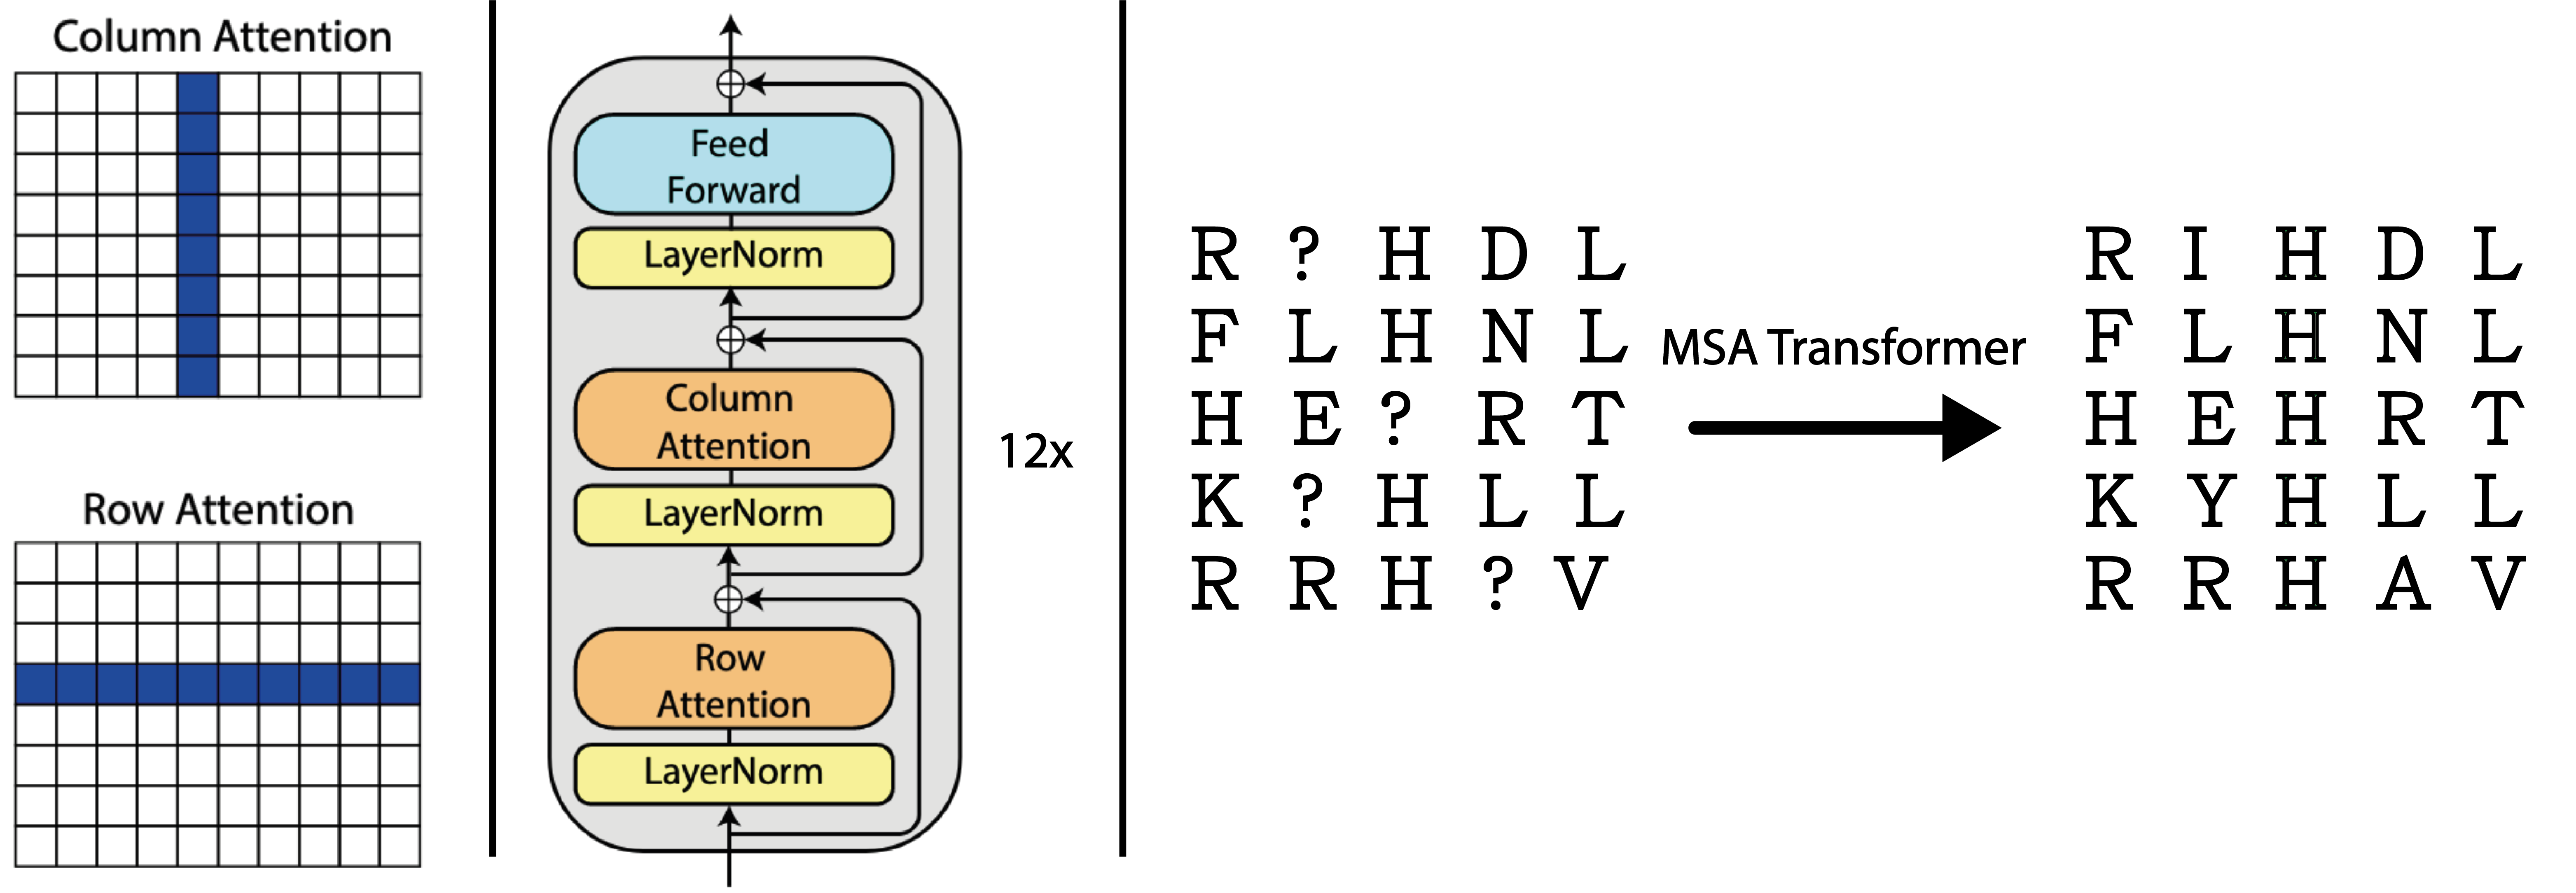
\includegraphics[width=\textwidth]{MSA_transformer.png}
\caption{A single MSA transformer block (left), column, and row attention are followed up by a feedforward layer. The MSA transformer training objective (right), amino acids are masked out at random in the MSA and the training objective is to recover the missing tokens. Adapted from \cite{rao2020transformer}.}
\label{fig1}
\end{figure*}

\section{Data Pre-processing}
We want to train a binary classifier to predict whether two proteins interact, or do not interact, given a sequence embedding from the MSA transformer. First, we need a suitable dataset containing positive and negative PPI examples. Then we need to generate MSAs for this dataset and extract embeddings from the MSA transformer.

\subsection{Dataset}
The current state-of-art PPI prediction software that can predict PPIs from sequences is D-SCRIPT (Deep Sequence Contact Residue Interaction Prediction Transfer) \cite{sledzieski2021d}. D-SCRIPT uses a pre-trained pLM to generate an interpretable contact map and to classify protein pairs as interacting or non-interacting. The D-SCRIPT training dataset contains 38,345 human PPIs which we can use for training our model. We can also use the results achieved by D-SCRIPT as a benchmark for our architectures.

\subsection{MSA Generation}
The first step in our pre-processing pipeline is to take the sequences from the dataset and start generating MSAs. For this task, we use the software tool mmseqs2 \cite{steinegger2017mmseqs2}. Using mmseqs2, we can perform a sensitive and high-speed database search of Uniref100 \cite{suzek2015uniref}; this is a database containing protein sequences of various genomes pre-clustered for sequence similarity. A Smith-Waterman algorithm is used to find similar sequences and align them; this results in a massive list of thousands of protein sequences. These protein sequences are then filtered on sequence diversity, resulting in a minimum of 300 protein sequences per protein domain. The obtained MSAs can then be used as an input for the MSA transformer to extract the embeddings.

\subsection{MSA Embedding Extraction}
We use the final layer (layer 12) to extract embeddings for our MSAs. This results in an embedding of sequence length $L$ by the number of sequences in the MSA $M$ and an embedding dimension of $d = 768$. We only keep the first row of the output, which gives us the embedding for the query sequence. This embedding can then be used to train a binary classifier to predict whether a pair of proteins interact or not. An overview of the embedding generation pipeline can be seen in Figure \ref{fig2}.

\begin{figure*}[t]
\centering
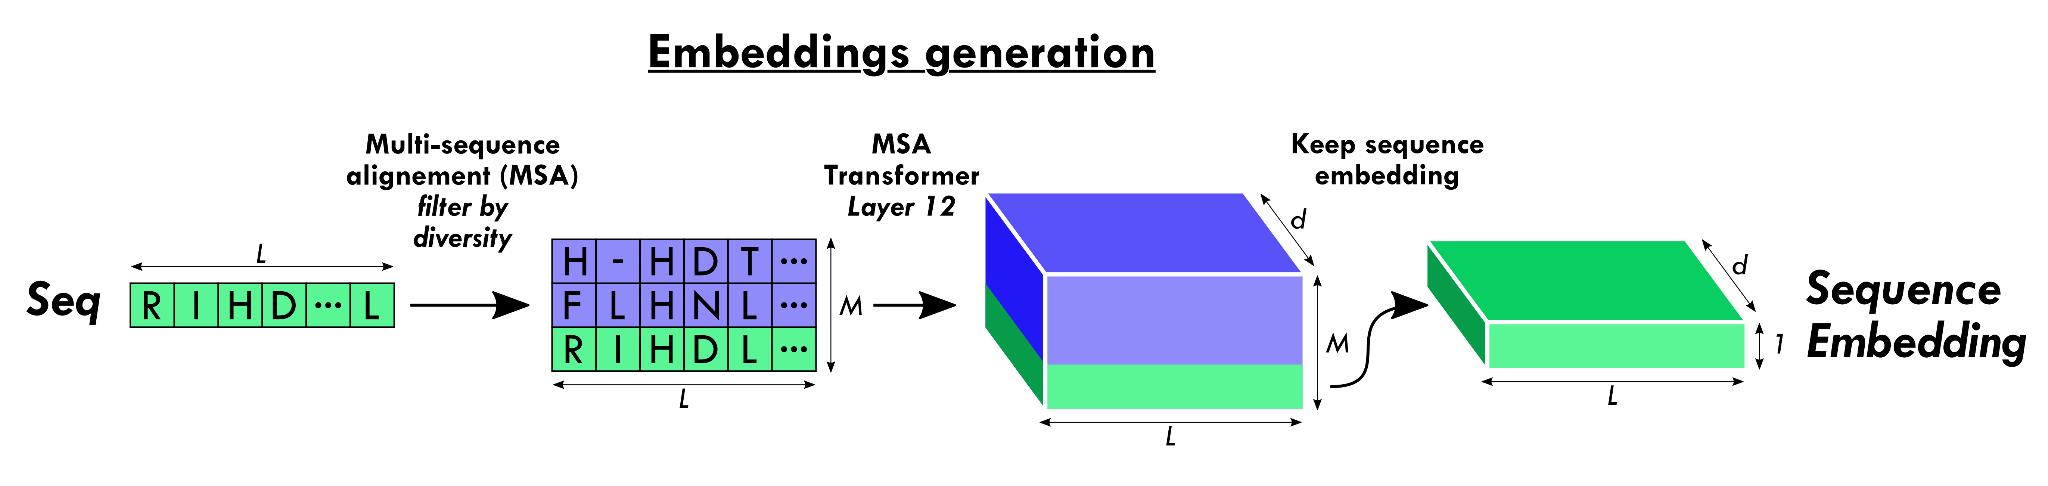
\includegraphics[width=\textwidth]{emb_gen.png}
\caption{The embedding generation pipeline. First, for each sequence with length $L$, an MSA is generated using a database search of UniRef using mmseqs2. Next, the MSA is filtered on sequence diversity resulting in an $L \times M$ tensor where M is the number of sequences in the MSA. This MSA is used as an input into the MSA transformer where the embedding of layer 12 is extracted, resulting in a matrix of $L \times M \times d$ (where $d = 768$). Finally, we store the embedding of the query sequence resulting in an $L \times d$ sequence embedding.}
\label{fig2}
\end{figure*}



\section{Input Visualization}

To better understand the information contained in the input, a thorough data analysis of the MSA embeddings is performed. The paper introducing the MSA Transformer \cite{rao2021msa} contains several analyses showing that information about the protein's properties can be extracted from the intermediate embeddings of the model.

Nonetheless, we conducted on our own a series of data visualizations to get familiar with the embeddings and test if they could hold information relevant for our specific task.

\subsection{Dimension Reduction}

We used Uniform Manifold Approximation and Projection (UMAP) \cite{mcinnes2018umap} to reduce the dimension of the embeddings from 768 dimensions to 2 while preserving their structure. We treated the vector corresponding to each amino acid as independent of the others in the same sequence. 

The results for layer 12 of the MSA Transformer are shown in Figure \ref{fig_umap_lay12}, where each letter corresponds to an amino acid. Not surprisingly, we observe clusters corresponding to each amino acid, i.e., we can almost perfectly recover the input letters in the embeddings.

\begin{figure*}[ht]
\centering
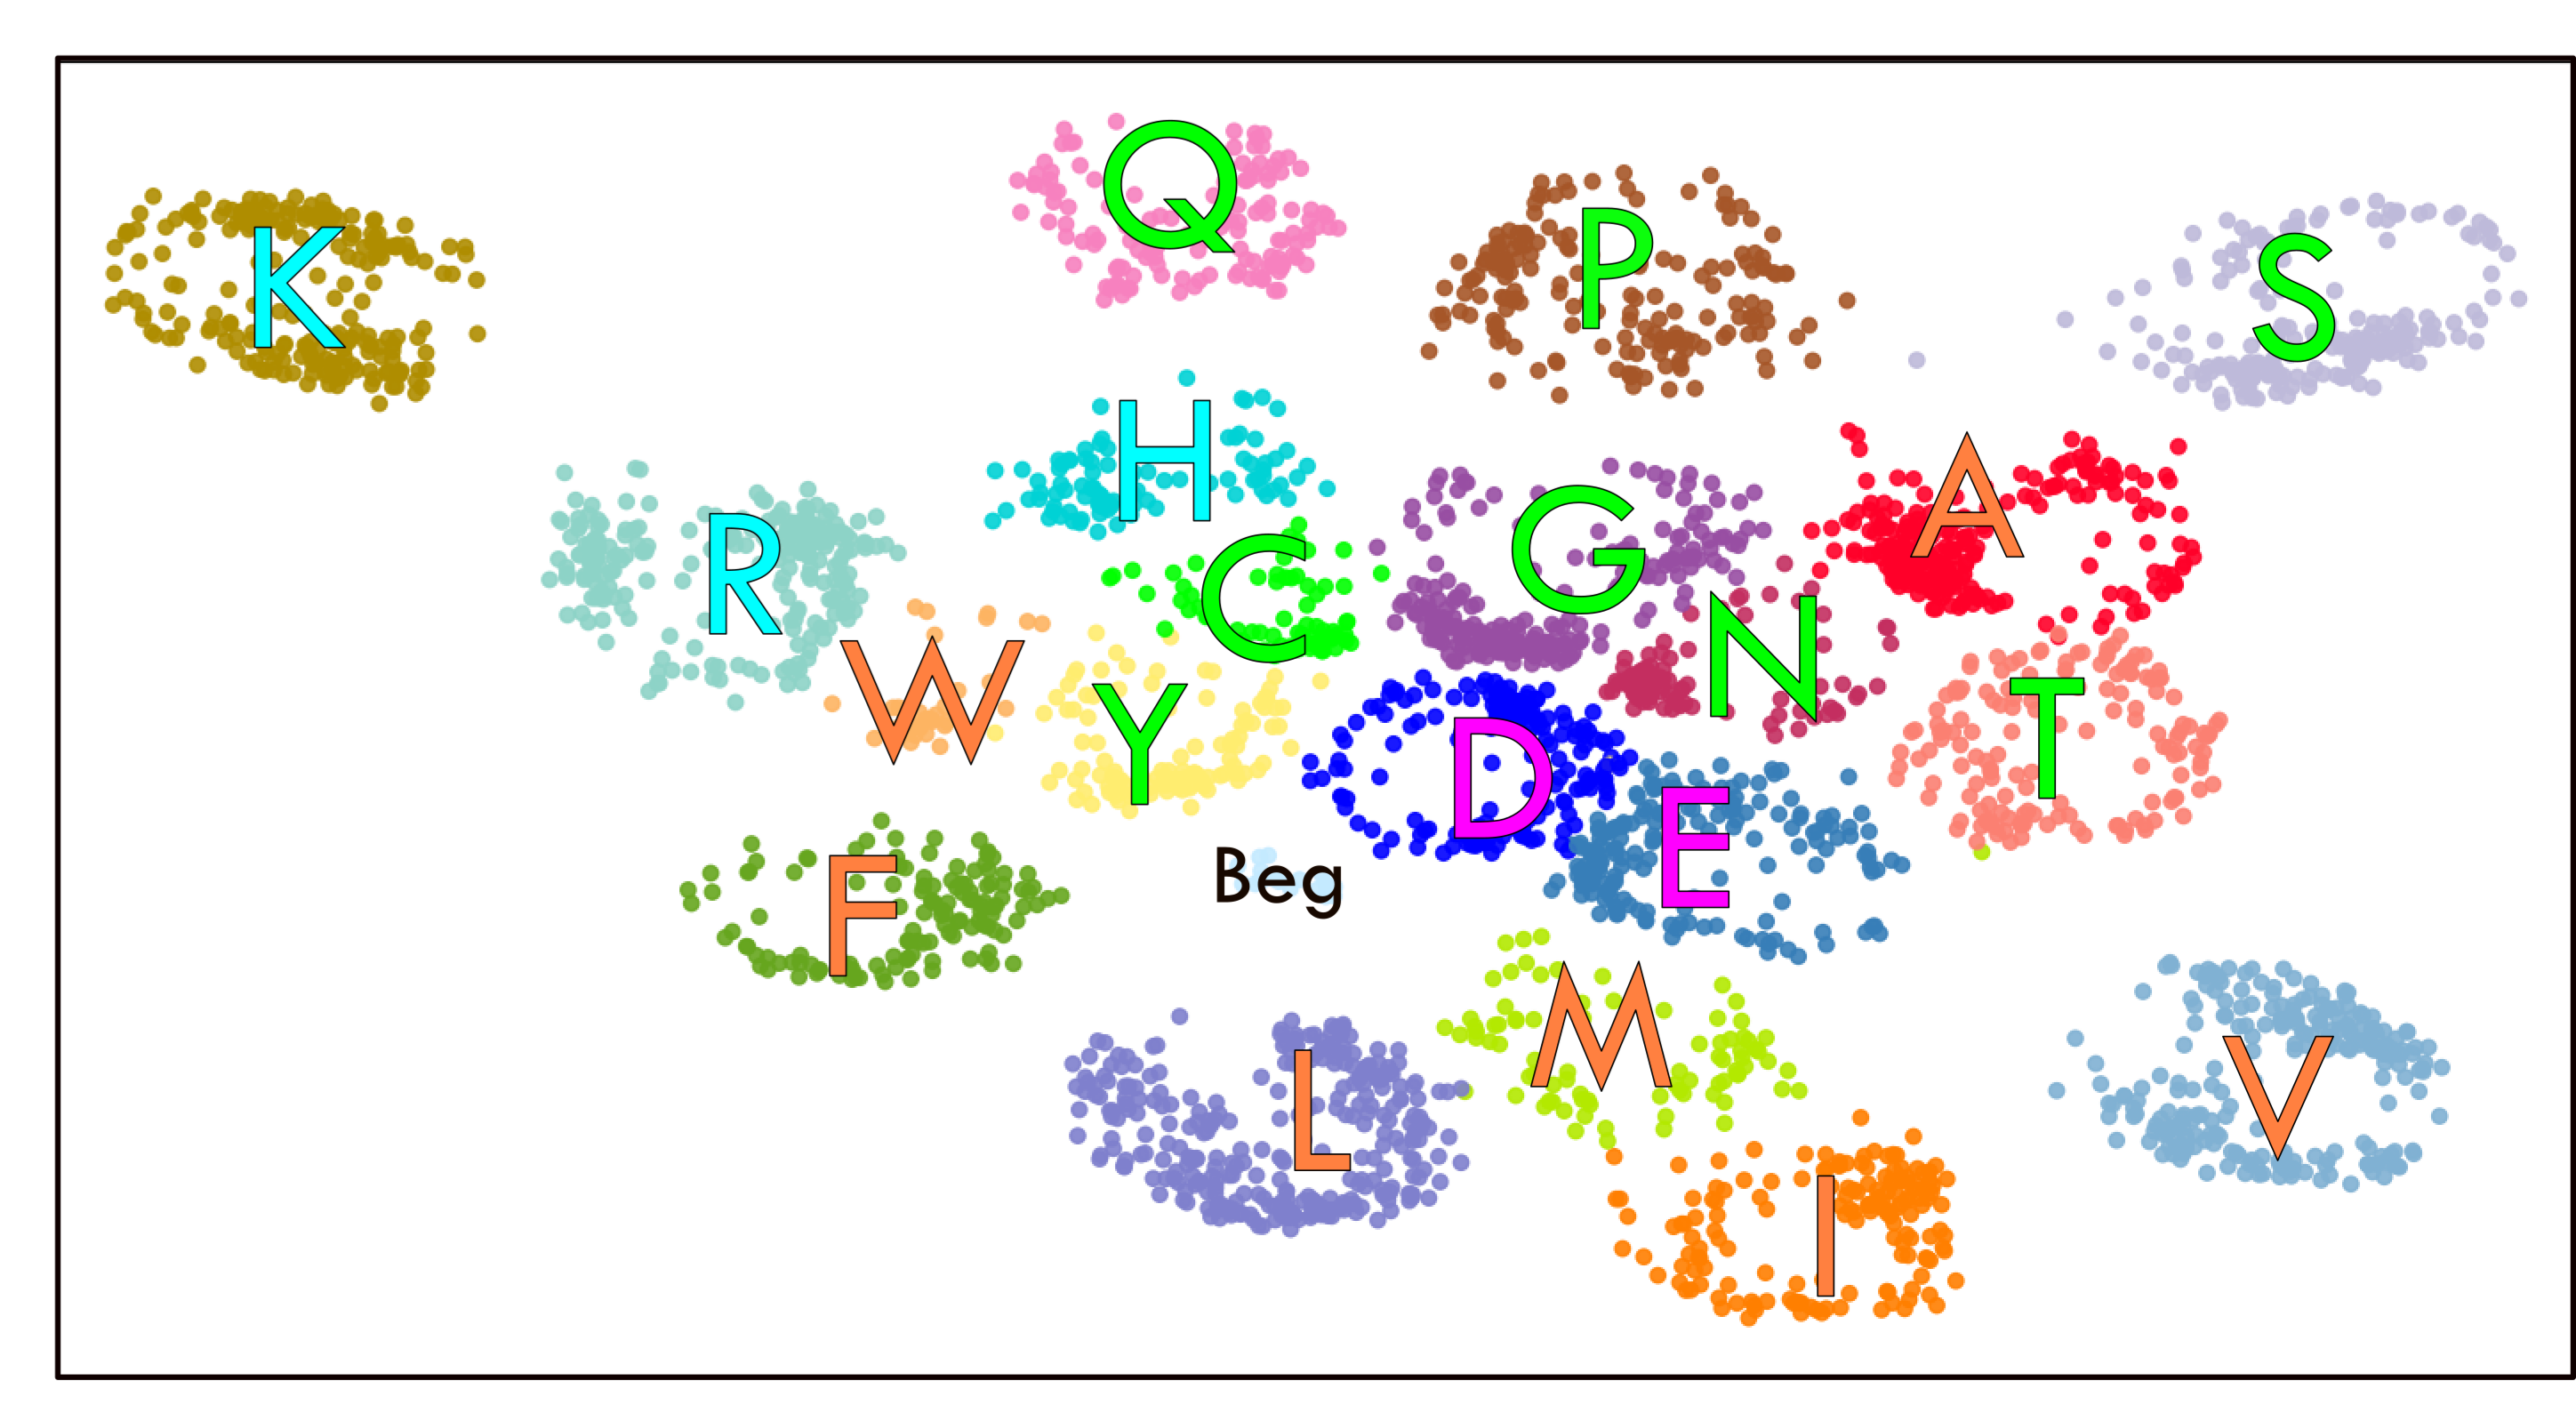
\includegraphics[width=\textwidth]{images/layer_12_umap.png}
\caption{Visualization of the embeddings from the layer 12 of the MSA Transformer after reducing the dimension with UMAP. Each letter corresponds to an amino acid, \texttt{Beg} corresponds to the token at the beginning of the sequences. The color of each letter corresponds to the chemical family of the amino acid, according to figure \ref{fig_amino_acid_families}. }
\label{fig_umap_lay12}
\end{figure*}

\begin{figure*}[ht]
\centering
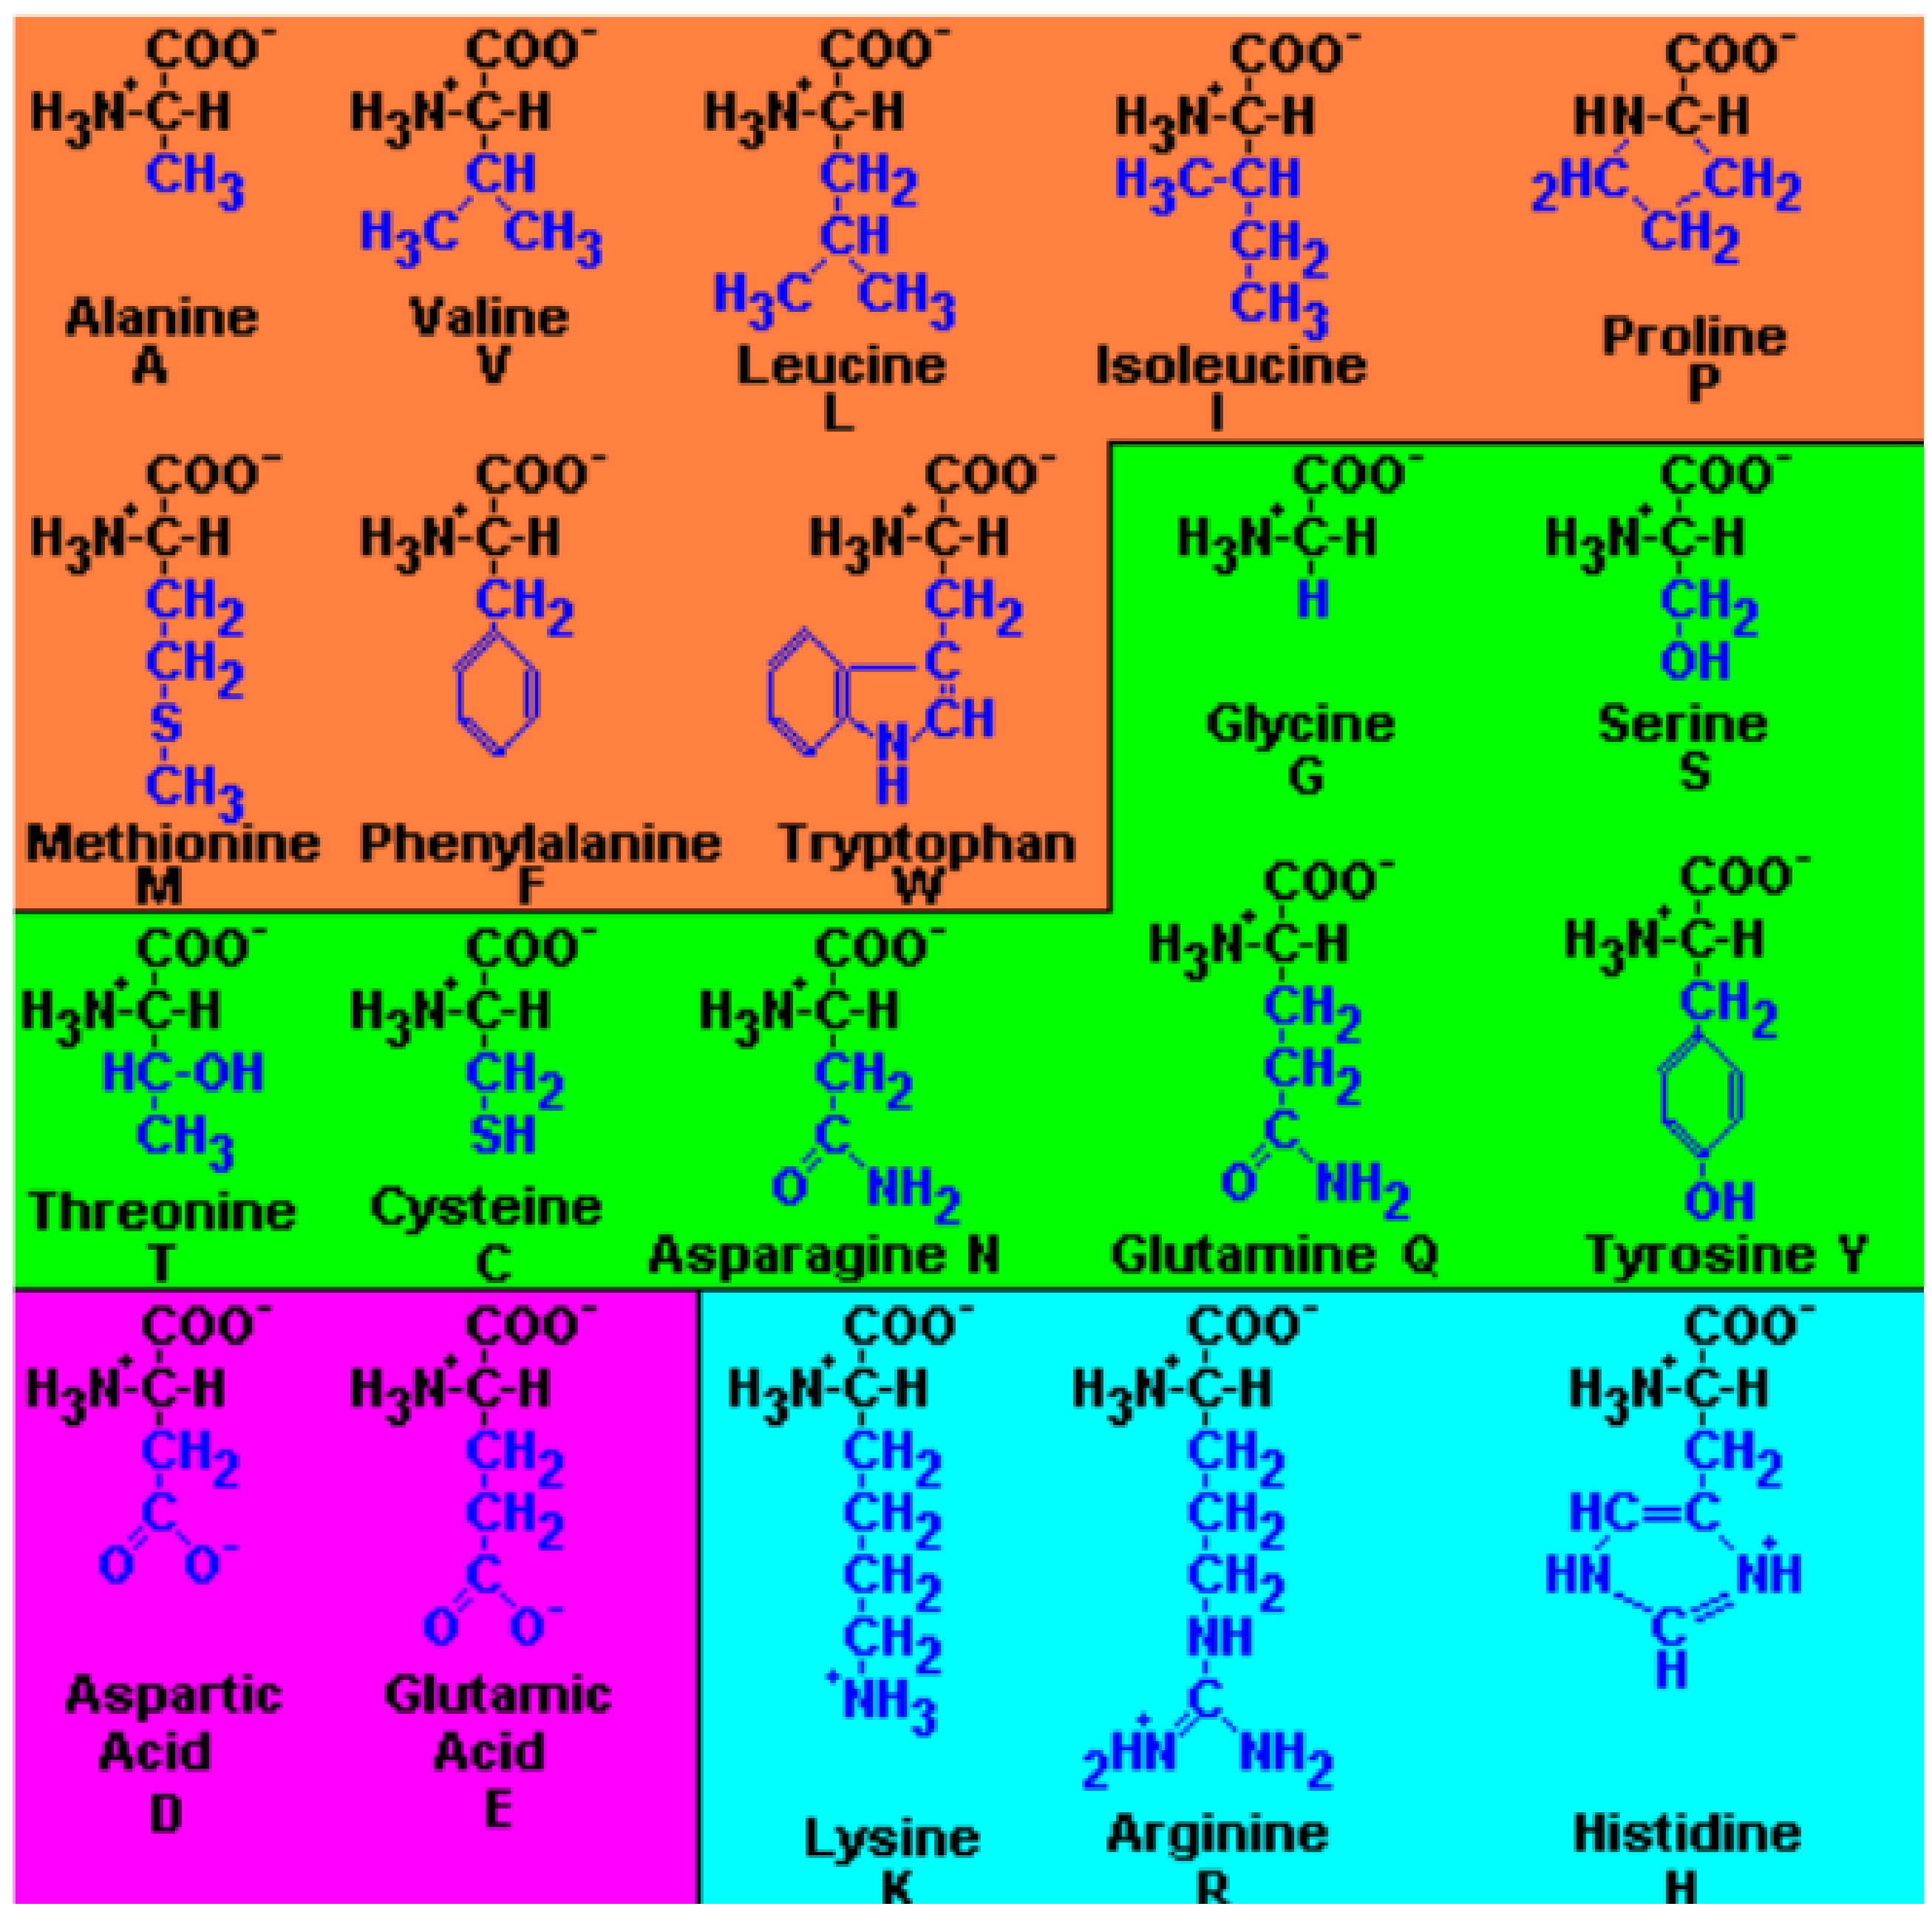
\includegraphics[width=0.4\textwidth]{images/ac_families.png}
\caption{The 20 amino acids used to form proteins. They are organized according to their chemical properties: orange are hydrophobic, green are hydrophilic and neutral, magenta are hydrophilic and acid, blue are hydrophilic and basic. }% Table taken from  }
\label{fig_amino_acid_families}
\end{figure*}

Nonetheless, one interesting point we discovered is that the relative position of the clusters is not random. Their positions seem to encode information about the chemical property of each amino acid, as depicted in Figure \ref{fig_umap_lay12}, where the color of the amino acids corresponds to their chemical properties. For instance, the light blue color corresponds to positively charged amino acids.

This structure is not surprising given the pretraining of the MSA Transformer. To predict a masked token, it makes sense that the intermediate representation is correlated with chemical properties: amino acids with similar effects tend to appear in a similar context. This can be seen as synonymy for words. 
The Figure \ref{three_layers_umap} shows that the structure seems globally conserved through the depth of the Transformer. We hypothesize that dimension reduction is only able to show the coarse-grained structure of the underlying space; the fine-grained details appearing during the processing by the Transformer may not be visible here.

\begin{figure*}[ht]
\centering
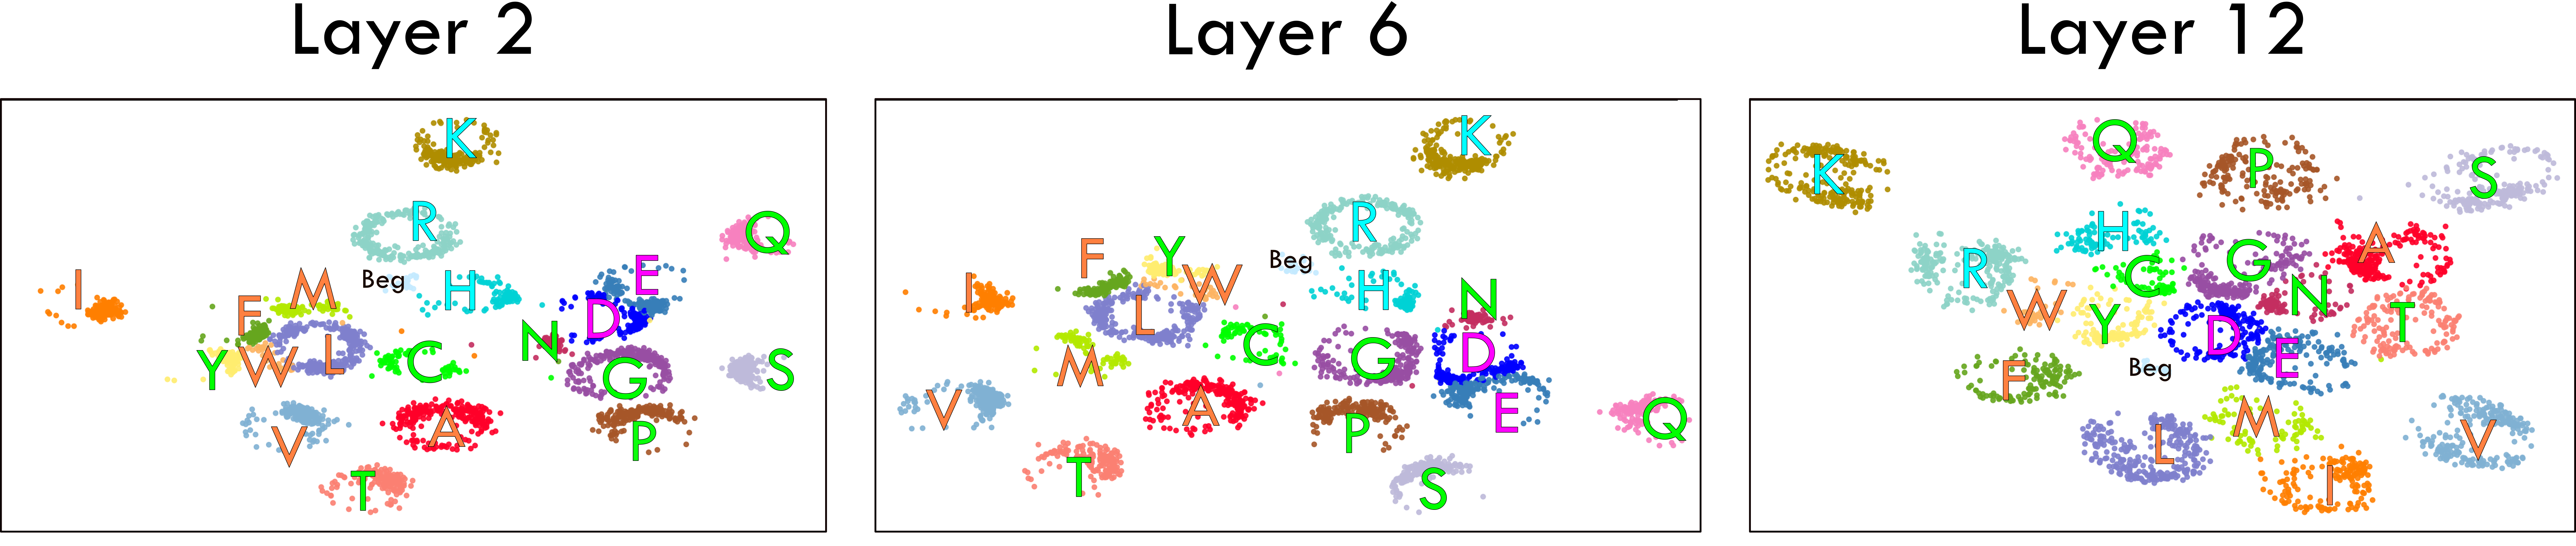
\includegraphics[width=\textwidth]{images/all_three_layers_strcut.png}
\caption{Visualizations of the embeddings through dimension reduction with UMAP for 3 different layers of the MSA Transformer. }
\label{three_layers_umap}
\end{figure*}

\subsection{Secondary Structure Prediction} \label{sec_struct_section}

As described in the introduction, the complexity of proteins lies in the fact that their function comes from structure. The structure can be subdivided into roughly three scales; the primary, secondary and tertiary structure. The primary structure is the order of the amino acids. The secondary structure is the formation of small structural elements from the primary structure, namely $\alpha$-helices or $\beta$-sheets. In turn the secondary structural elements fold into a larger structural complex which is becomes the final protein structure.

After observing meaningful structures related to the chemical properties of individual amino acids, we experimented with the next scale: the secondary structure. It corresponds to parts of proteins organized in either helices or flat patterns formed by a succession of 180° turns. These two are respectively called $\alpha$-helices and $\beta$-sheets. The presence or absence of their substructure plays an essential role in the protein's function. For instance, $\alpha$-helices can be markers of proteins going through the membranes of cells.
However, predicting where these patterns will emerge in the proteins is already a complex problem and there is no straightforward
way to link sub-sequences of amino acids to their secondary structure. 

To experiment if this crucial information was present in the embeddings, we use the online service \emph{Jpred} \cite{cole2008jpred} to get the secondary structure of a test set of sequences.

In general, we did not observe a strong correlation between secondary structure and the position in the embeddings space, except for certain amino acids, as visible in Figure \ref{zoom_umap_sec_struct}. We can observe that the position inside the cluster is correlated with the secondary structure they form. 

\begin{figure*}[ht]
\centering
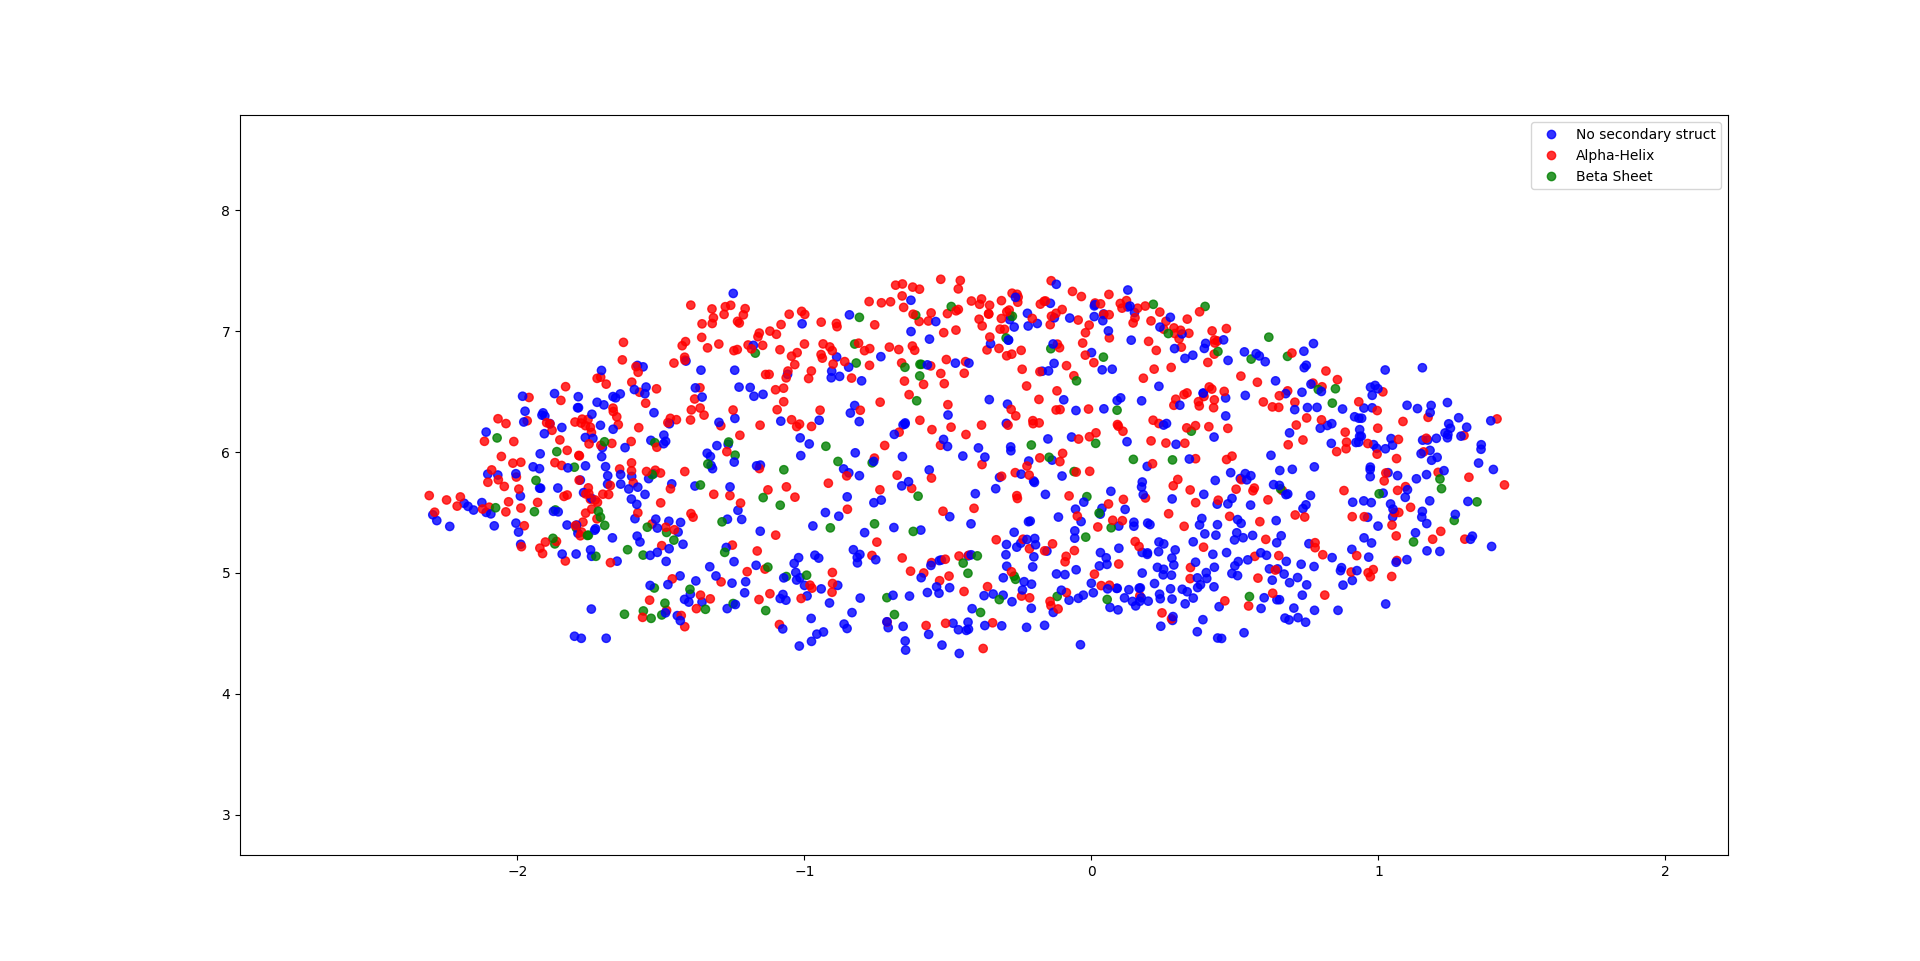
\includegraphics[width=0.8\textwidth]{images/sec_struct_zoom.png}
\caption{Zoom on a cluster of a UMAP visualization for layer 12. The color of the points corresponds to the secondary structure the amino acid is forming: red corresponds to $\alpha$-helices, green to $\beta$-sheets, and blue to no particular secondary structure. }
\label{zoom_umap_sec_struct}
\end{figure*}


\begin{figure*}[ht]
\centering
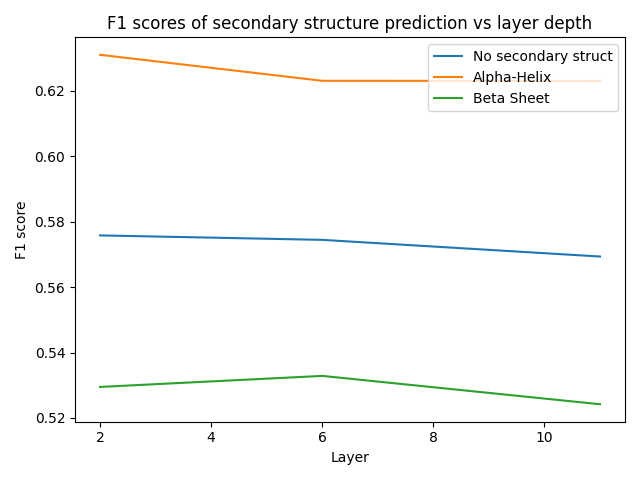
\includegraphics[width=0.5\textwidth]{images/plots_sec_pred_logistic_regression.png}
\caption{Performance of a linear probe trained to predict the secondary structure from the MSA Transformer embeddings at different layers. The F1 score is above 0.5 for all layers and classes. This demonstrate an ability to predict these labels much better than random guess. }
\label{plot_f1_scores_linear_probe_sec_struct}
\end{figure*}

To corroborate these qualitative results, we trained a linear classifier to predict the secondary structure of an individual amino acid from its embeddings taken from different layers of the MSA Transformer. The performance for three layers is shared in Figure \ref{plot_f1_scores_linear_probe_sec_struct}. We observe a performance of 71\% accuracy on a test set with balanced classes (36\% if we use only the tokens as input).
This means that the embeddings of individual amino acids contain meaningful information about their context. This is coherent with a similar experiment conducted in the MSA Transformer \cite{rao2021msa}, but here, we obtain the results for several layers. The layer depth does not seem to play an important role in the precision of the prediction. We hypothesize that the secondary structure is a low-scale pattern already encoded since the first layers.


\section{Methods}
%\todo[inline]{A few introductory sentences. (at the end)}



\subsection{Baseline Models}
To compare how simple model architectures perform against more complex ones, a simple MLP is trained using the MSA transformer embeddings to predict protein binding. We call this simple MLP model our baseline model.


\paragraph{Dataset}
Although we keep only the first embedding from each MSA, the dataset is still enormous -- pairs of sequences can be up to $1600$ amino acids long while each amino acid is represented as a vector of dimension $d = 768$. Because we want to have a simple baseline that is not computationally demanding, the original dataset must be adapted. For this purpose, mean or max poolings are applied to the embeddings along the length dimension, resulting in vectors of size $d$. Depending on the type of pooling, we get two baseline models: baseline-max and baseline-mean. The corresponding compressed embeddings are concatenated and fed into one of the baseline models to predict whether a pair of proteins interact.


\paragraph{Model architecture}
The design of baseline models is also kept uncomplicated. They are just vanilla multilayer perceptrons (MLPs), consisting of multiple blocks stacked on top of each other. All but the last block, consists of sequentially applied a linear layer, a batch normalization \cite{ioffe2015batch}, a ReLU \cite{agarap2018deep} activation function, and dropout \cite{srivastava2014dropout}. On the other hand, the last block contains only a linear layer and sigmoid \cite{nwankpa2020activation} activation function. Dropout is added to prevent overfitting, while batch normalization allows faster and more stable training. The output of the model represents the probability of protein binding. Their architecture is described in Figure \ref{fig:baseline_archi}.

\paragraph{Experimental setting}

Both baseline models have $4$ layers with a hidden dimension of $128$. They are trained for $400$ epochs, with batch size of $128$, Adam optimizer \cite{kingma2015adam}, initial learning rate of $10^{-3}$, weight decay of $5 \cdot 10^{-4}$, dropout of $0.3$, and Focal Loss hyperparameters $\alpha=0.1$ and $\gamma=2$. During training, the learning rate is modified according to a polynomial learning rate policy \cite{mishra2019polynomial}. 




\begin{figure*}[ht]
    \centering
    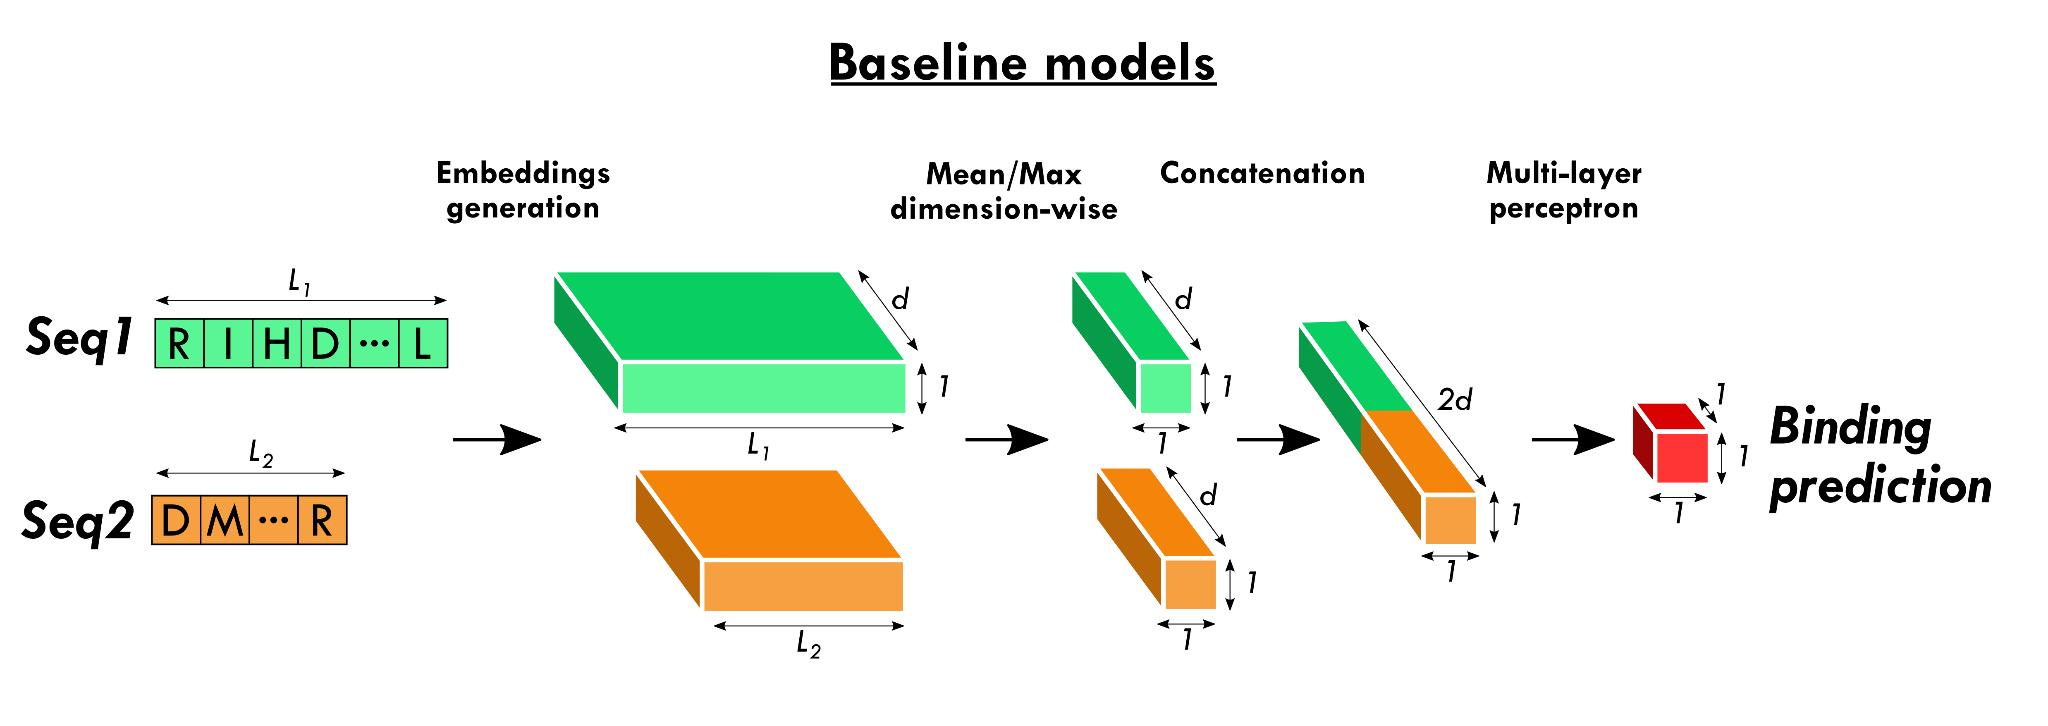
\includegraphics[width=\textwidth]{baseline_models.png}
    \caption{The architecture of the baseline models.}
    \label{fig:baseline_archi}
\end{figure*}






\subsection{Transformer Model}

Using some aggregation function such as mean or max-pooling to reduce the dataset is computationally efficient but may lack subtlety. If the latent space of the MSA embeddings is entangled, then the pooling operations may not select important features. Since the MSA transformer is not constructed with latent space disentanglement in mind, it would be an error not to train a model to look at the entire sequences. We chose to use transformers \cite{NIPS2017_3f5ee243} over LSTMs \cite{hochreiter1997long} due to them being more parallelizable and the fact that the attention mechanism offers a convenient inductive bias for our task.
First, the individual amino acids can look at other amino acids from the same sequence to obtain information about %\todo[inline]{we don't talk about secondary structure before this, should I drop it? -> Alexandre : I added a ref to the point I talk about sec structure, it's cool to link parts together !} 
potential secondary structure (see section \ref{sec_struct_section} for more details on this). In higher layers, amino acids from one sequence can look at amino acids of the other sequence and select for interesting properties. One could easily imagine an attention head that lights up if two amino acids have a different polarity as useful. \\
We encode our task in the same manner as the next sentence prediction pretraining task of BERT \cite{devlin-etal-2019-bert}. The final sequence fed to the transformer is a classifier token, the first protein, a separator token, the second protein, and finally a separator token. As can be seen in Figure \ref{fig:transformer_arch} two embeddings are added to the original token embeddings. Positional encoding is added to the entire sequence. Similarly, two different embeddings are added depending on which protein the token belongs to. After passing through the transformer, the classifier token is fed through a simple predictor to obtain the probability of interaction.

\begin{figure*}[ht]
\centering
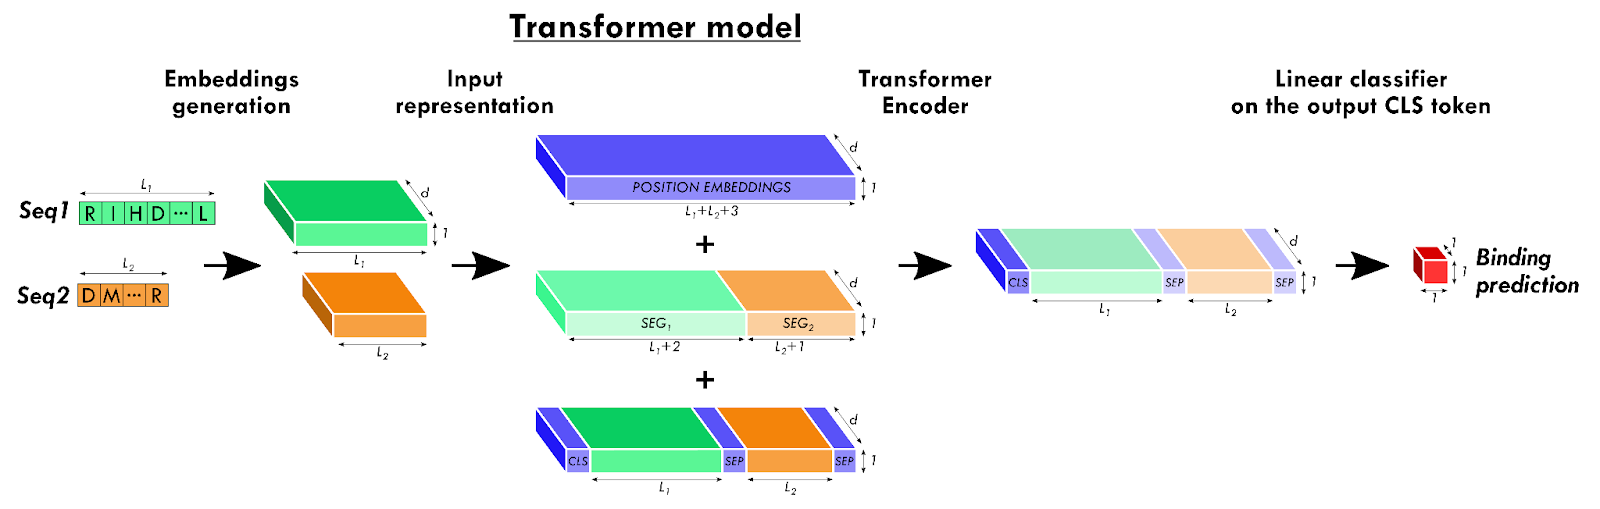
\includegraphics[width=\textwidth]{images/transformer architecture.png}
\caption{Graphical representation of the transformer architecture used.}
\label{fig:transformer_arch}
\end{figure*}


\paragraph{Dataset}
Similar to the baseline dataset we only keep the first embedding from each MSA, this time however we conserve the whole sequence. The average sample length is 753 tokens.


\paragraph{Experimental setting} 

The transformer model has 4 layers with a dimension of 768, a feed-forward dimension of 2048 and 8 attention heads. For the optimization process we followed the original transformer recommendations. We used Adam with a simulated batch size of 512 and an additional learning rate scheduler given by the formula:
\begin{align*}
    lrate = d_\text{model}^{-0.5} \cdot \text{min}(step\_num^{-0.5}, step\_num \cdot \\ warmup\_steps^{-1.5})
\end{align*}




\subsection{Focal Loss}

Due to the high imbalance of the dataset -- there are around nine times more negative instances than positive ones -- additional measures have to be considered. Without adapting the loss function and balancing the training data, the model might not learn anything. To avoid this problem, Focal Loss \cite{lin2017focal} is employed, which mitigates the class imbalance problem. Focal Loss calculates the loss of a single example in the following manner:

\begin{align}
    p_t &= 
    \begin{cases}
     p & \text{if } y = 1  \\
     1 - p & \text{otherwise},
    \end{cases} \\
    FL(p_t) &= -\alpha_t (1 - p_t)^{\gamma}\log(p_t),
\end{align}

\noindent
Where $p$ is the prediction of the model, $p_t$ is the confidence of the model in the correct label $y$, and $\alpha$ and $\gamma$  are hyperparameters of the loss. $\alpha$ makes the minority class more important by increasing its value compared to the majority class. Higher values of $\gamma$ places less importance on samples that are already correctly and confidently classified. In the case of binary classification, $\alpha$ usually denotes the weight of the negative class; therefore, $1 - \alpha$ is the weight of the positive class.



\section{Metrics}

To compare models fairly, we must use a metric adapted to the problem at hand. An important property of the metric to be considered is that it should give more importance to predicting the minority class with high precision, rather than with high recall \cite{metrics}. The reason is simple: the model's prediction will have to be experimentally verified, which is a costly procedure.

One idea would be to use the Precision score as a metric. However, such a metric is not adapted, as a model predicting a match for only trivial interactions would get too high of a score. To counter this, Recall should be taken into consideration. Comparing models using two metrics is not convenient, which led to consider the F$_\beta$-score (which is a harmonic mean of Precision and Recall, giving more importance to Precision or Recall depending on the value of $\beta$). However, this metric is still not adapted because it is unclear what the most relevant value of $\beta$ is to choose. The F$_\beta$-score is computed with the model's binary predictions rather than probabilistic ones (using a threshold value). This threshold value is model dependant, which makes it difficult to standardize.

Instead, other models such as the D-SCRIPT models evaluate their models using a combination of metrics:  AUPR, Precision, Recall, AUROC. Precision and Recall provide an easily interpretable metric (although sometimes misleading). AUPR and AUROC are Area Under the Precision-Recall curve and Area Under the Receiver Operating Characteristic curve respectively. To overcome the model-dependent threshold issue, one solution is to plot the points (Precision, Recall) on a graph for every thresholds. Such an operation results in the Precision-Recall curve. Suppose instead we plot Recall (also called True Positive Rate) with respect to the False Positive Rate $= \frac{FP}{FP+TN}$ (probability that a false alarm will be raised: that a positive result will be given when the true value is negative). In that case, we get the Receiver Operating Characteristic curve. In both cases, the higher the curve, the better.

Because AUPR depends on Precision, and AUROC does not, we give in our model comparison more importance to AUPR than AUROC. Furthermore, recent works have shown that ROC can give overly-optimistic scores for classifiers when applied to imbalanced data. In contrast, PRC provides better insight into the performance of a classifier by focusing on the minority class \cite{limit_ROC}. On the \emph{H. sapiens} testing set that we are evaluating our model on, there is a ratio of around 1:10 between positive samples (interaction) and negative samples (no interaction), as is the case in most of our data since most of the proteins do not interact.

It is important to note that we should be careful when comparing areas under the curve values. Indeed, this value reflects the performance of different models (tuned with different thresholds), not one model's performance. As a result, reducing the curve to a single number gives an average performance overall thresholds. However, some of these regions might not be of interest. For instance, in our application, the model's performance on a low threshold (i.e. when Recall is high) is of much less importance to us than the performance of the model on a high threshold (i.e. when Precision is high). However, the area under the curve gives equal importance to both. This is why certain works use partial AUC by considering only the area under a particular region of the curve. Despite this variant being more adapted to our application, the other works do not make use of it, and thus we cannot use it to compare models.

This is why, in addition to the four metrics previously mentioned, we provide in Figure \ref{fig:curves} the plotted Precision-Recall curve of our models.

\begin{figure}
     \caption{The test set precision-recall curves of our models}
     \label{fig:curves}
     \centering
     \begin{subfigure}[b]{0.5\textwidth}
         \centering
         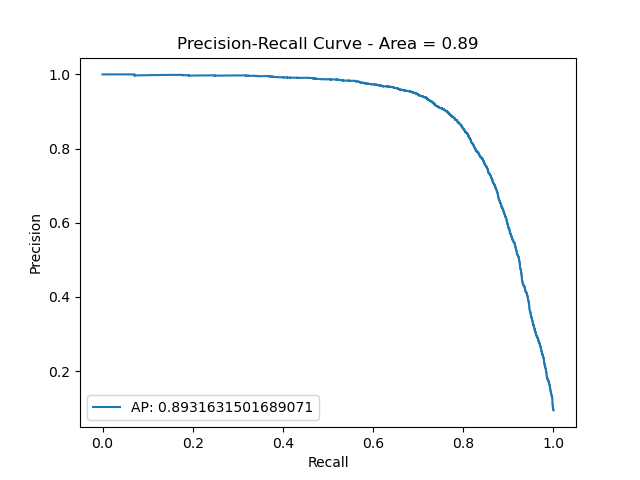
\includegraphics[width=\textwidth]{images/baseline_max_pooling.png}
         \caption{Precision-recall curve of the max-pooling baseline}
         \label{fig:max_pooling}
     \end{subfigure}
     \hfill
     \begin{subfigure}[b]{0.5\textwidth}
         \centering
         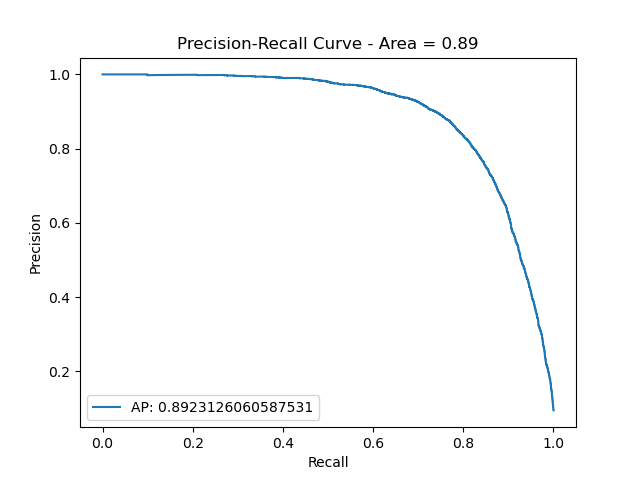
\includegraphics[width=\textwidth]{images/baseline_mean_pooling.png}
         \caption{Precision-recall curve of the mean-pooling baseline}
         \label{fig:mean_pooling}
     \end{subfigure}
\end{figure}

\section{Results}

%\todo[inline]{A few introductory sentences. (at the end)}

%\paragraph{Experimental setting}
To assess the performance of our models, we compare the baseline model on the max-pooled dataset, the baseline model on the mean-pooled dataset, and the transformer model with D-SCRIPT.

Since precision and recall require binary predictions, predictions of the models are thresholded with the threshold of $0.5$. Results are reported in the table \ref{table_result} for the best version of each model considering validation AUPR for the baseline models and validation AUROC for the transformer model.

%\todo[inline]{We use the same training and testing set of human (\textit{H. sapiens}) proteins as D-SCRIPT paper. CHECK IF THIS IS CORRECT? Yes we use the same training and testing set, however in the dscript paper they use 5 fold cross validation on the test set, so direct comparison might not be possible} Furthermore, we split training dataset in training and validation set according to $85/15$ ratio.




%\paragraph{Evaluation}
%When evaluating the models, we are principally interested in performance on the positive class since testing whether a pair of proteins interact is very expensive. Therefore, we decided to compare models according to the area under the precision-recall curve (AUPR), the area under a receiver operating characteristic curve (AUROC), precision, and recall. D-SCRIPT is also evaluated with these metrics, so our approaches are directly comparable. 
%\todo[inline]{Can be adapted according to what Loic writes.}



\begin{table}[h!]
    \caption{Metrics comparison of our models and D-SCRIPT on the \textit{H. sapiens} dataset.}
    \label{table_result}
    \centering
    
    \resizebox{\columnwidth}{!}{
    \begin{tabular}{ccccc}
        \toprule
        \textbf{Model} & \multicolumn{4}{c}{\textbf{Results}} \\
                 & AUPR & AUROC & Precision & Recall \\
        \midrule
        D-SCRIPT & 0.844 & 0.949 & 0.962 & 0.400  \\
        \midrule
        Baseline-mean & 0.892 & \textbf{0.976} & \textbf{0.981} & 0.500 \\
        Baseline-max & \textbf{0.893} & 0.972 & 0.976 & 0.600 \\
        Transformer & 0.839 & 0.963  & 0.514 & \textbf{0.878} \\
        \bottomrule
    \end{tabular}
    }
\end{table}

Due to the lack of resources, we did not use the same 5-fold cross-validation that was done for the D-SCRIPT results. We can see that the baseline models significantly beat the D-SCRIPT result for the AUPR metric, which is our most important metric, as explained earlier in section 5. All three models tried also beat the AUROC metric. Since they are threshold-dependent, the precision and recall are less important and only added for completeness.

\section{Future Work}
Some additional models should be trained to explain precisely why the simpler baseline models outperform the transformer. Firstly the transformer should be used in the same context as the mean and max pooling. That is to say that both protein sequences should be fed one at a time through the transformer to obtain fixed-length embeddings, then those two embeddings are concatenated and fed through the MLP prediction head. 

It would also be interesting to use the same transformer architecture as presented but use the baseline model instead of the simple prediction head; this will help pinpoint if the sequence reduction or prediction is the bottleneck.

If we want to keep the idea of the transformer looking at both sequences at the same time, it would be interesting to use a relative positional encoding \cite{shaw2018selfattention}. Another improvement would be, if available, to find an auxiliary loss that asks to predict which amino acid interacts with which. We hypothesize that such a loss would help the optimization process find better attention heads.

\section{Conclusion}
In this project, we demonstrated that tools initially developed for natural language processing can be successfully applied to predict the physical properties of amino acids sequences. We used the large pre-trained MSA Transformer to incorporate information from different but similar proteins. Thanks to interpretability techniques notably used in NLP, we showed that this prepossessing step seems to add to the raw sequences information relevant to the molecule's structure. These embeddings are computed for two sequences and fed to downstream models to predict protein-protein interaction. We found that a simple MLP was enough to obtain state-of-the-art results on a benchmark dataset for this task. The more complex Transformer architecture did not seem to add more precision. We explored some of the possible reasons in the section \ref{model_visu_section} of the appendix. 
We also propose improvements to the training procedure for the Transformer architecture.
This project allowed us to use our theoretical knowledge from deep learning applied to NLP to create a complex data pipeline, informed architecture choices, and a successful prediction tool to predict protein-protein interaction.

\vspace*{6cm}

\pagebreak
\section{Appendix}

\subsection{Code}

The code of this project is available on \emph{GitHub} at \url{https://github.com/axelmarmet/protein_transformer}.


\subsubsection{Sequence Visualizations} \label{full_seq_visu_section}

We were interested in visualizing the position of whole sequences in the embedding space.
To this end, we used the same preprocessing as the baseline model: we used max-pooling to obtain a fixed size vector representation of the whole sequence. Then we visualize the protein-protein interactions by creating a graph where two points are connected if and only if the two proteins interact. Nonetheless, this method didn't lead to informative hindsight, as visible in figure \ref{max_pooling_umap_graph}.

\begin{figure*}[ht]
\centering
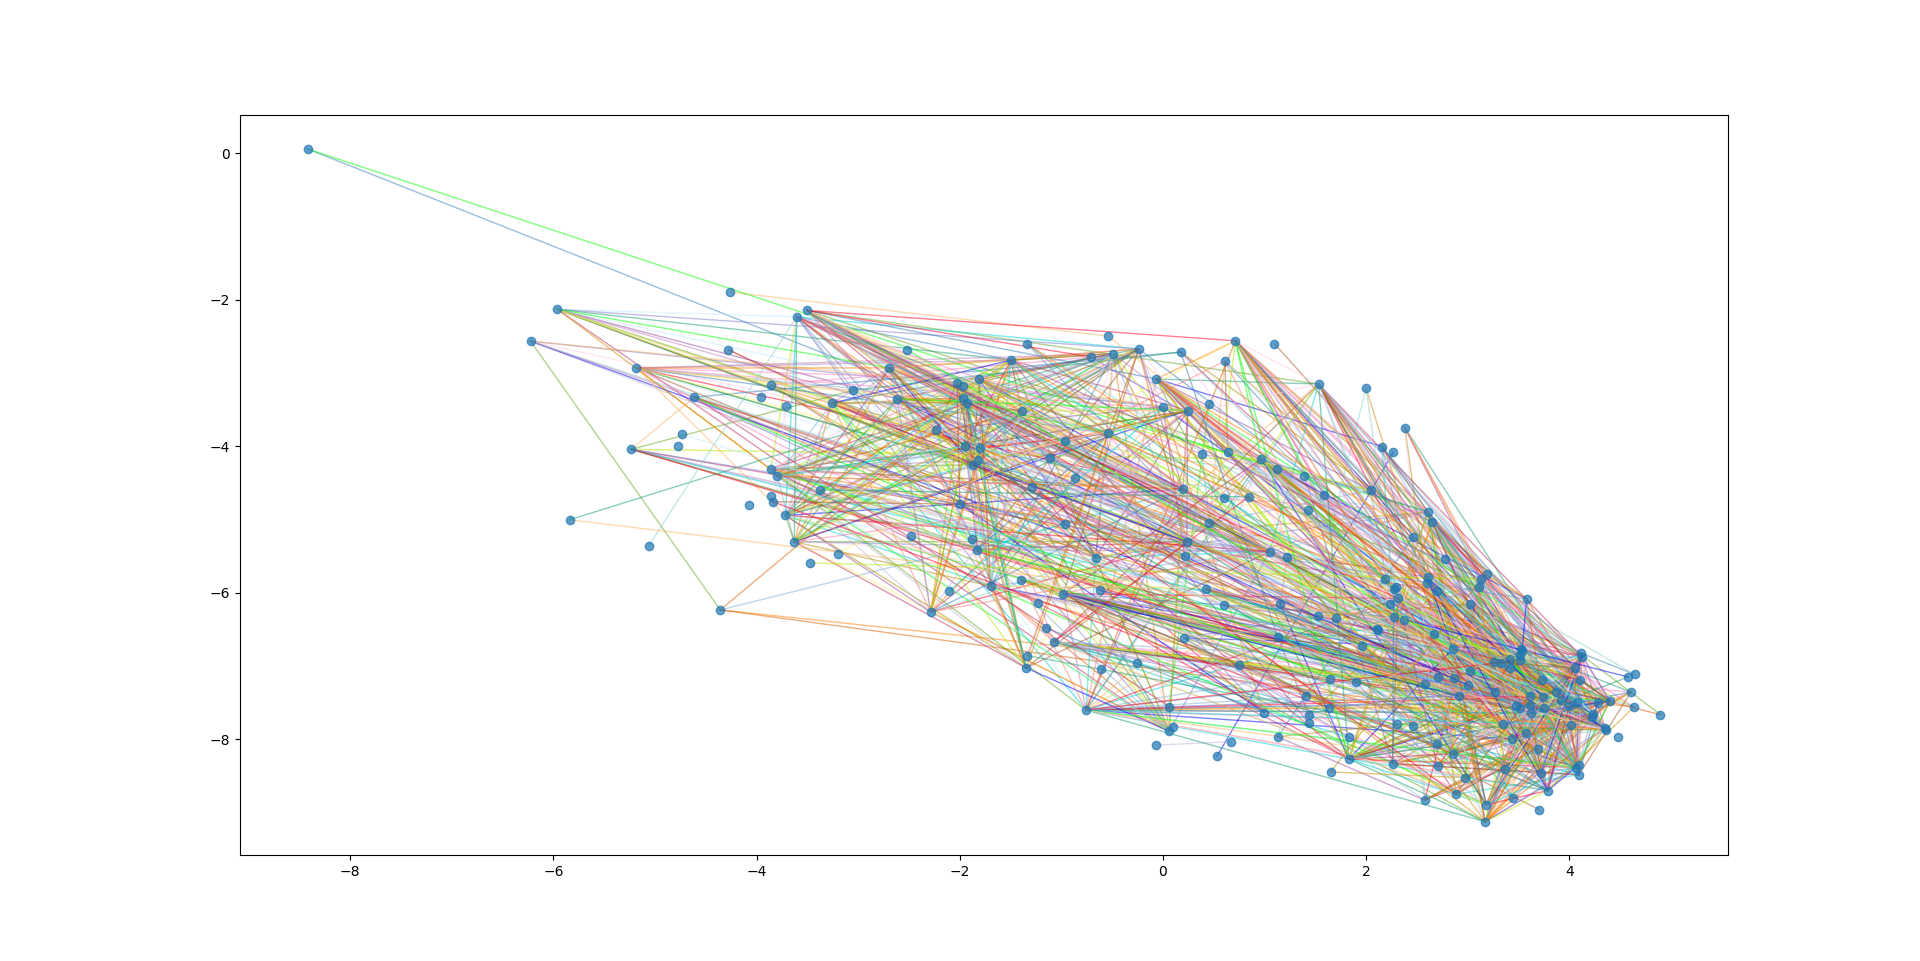
\includegraphics[width=0.8\textwidth]{images/graph_of_interaction_full_220_seq_lay11.png}
\caption{UMAP visualization of a protein interaction network. Each point corresponds to the embedding of a full protein computed with max-pooling. Two points are connected if and only if the two proteins they represent interact. }
\label{max_pooling_umap_graph}
\end{figure*}


\subsection{Model visualization} \label{model_visu_section}

We conducted a series of visualizations to understand the baseline model's excellent performance. Several reasons could explain this result; the most straightforward is the training time of the model. Compared to the computationally expensive Transformer model, we could train the simple multi-layer perceptron for an order of magnitude more epochs. 
Moreover, the max operation performed along the dimensions could be a simple way to compress the information of a sequence while keeping the information relevant to the binding properties of the complete protein, i.e., a cheap but effective hard-coded attention mechanism.
To test the former affirmation, we conducted visualizations of the trained MLP. We were not able to obtain clear-cut answers to the question presented above, and the following paragraphs are more exploratory than the description of rigorous experiments. Nonetheless, we think that the method was worth sharing, this is why we placed it in the appendix.


\subsubsection{Integrated gradient}

In the following experiment, we used our best model: the trained MLP with max pooling.

\paragraph{Case study}
As a case study for qualitative evaluation, we chose a protein complex part of our test set and a benchmark for protein-protein interactions \cite{hwang2010protein}. The complex is formed by four proteins, two human hemoglobin subunit alpha (HBA1) and two human hemoglobin subunit beta (HBB). The global structure of the complex can be thought of as a ring in the order HBA1-HBA1-HBB-HBB, as visible in figure \ref{3D_HBB_HBA1_complex}. Each protein interacts with the other and with itself: there are three types of two-protein interactions.

\paragraph{Visualization method}
For each input, we used Integrated Gradients \cite{sundararajan2017axiomatic} to obtain the attribution of each input dimension in the prediction. We then selected the five most important dimensions for each of the two proteins. For each of the chosen dimensions, we recover the corresponding position of the amino acid using the \texttt{argmax} operation. After identifying the "important" amino acids, we visualize them in the 3D structure of the complex.

\paragraph{Visualization results}

The distribution of the attribution given by the Integrated Gradients method can be observed in figure \ref{attribution_profils} for four inputs. We can observe that a few dimensions concentrate the most attributions: on average, 10\% of the dimensions concentrate 32\% of the total attribution (it makes sense to perform this computation given the completeness property of Integrated Gradients).  This partially justifies our choice to visualize the contribution of the top 5 dimensions for each sequence, even if we are aware that this technique does not give a full picture of the features exploited for the prediction. We can also see that the MLP does not seem to have learned the symmetry of the prediction. Indeed, because of the concatenation used to create the input, an artificial non-commutativity of the prediction is introduced. And, as the two first plots of the figure \ref{attribution_profils}  suggest, the attribution pattern is not symmetrical. 

\begin{figure*}[ht]
\centering
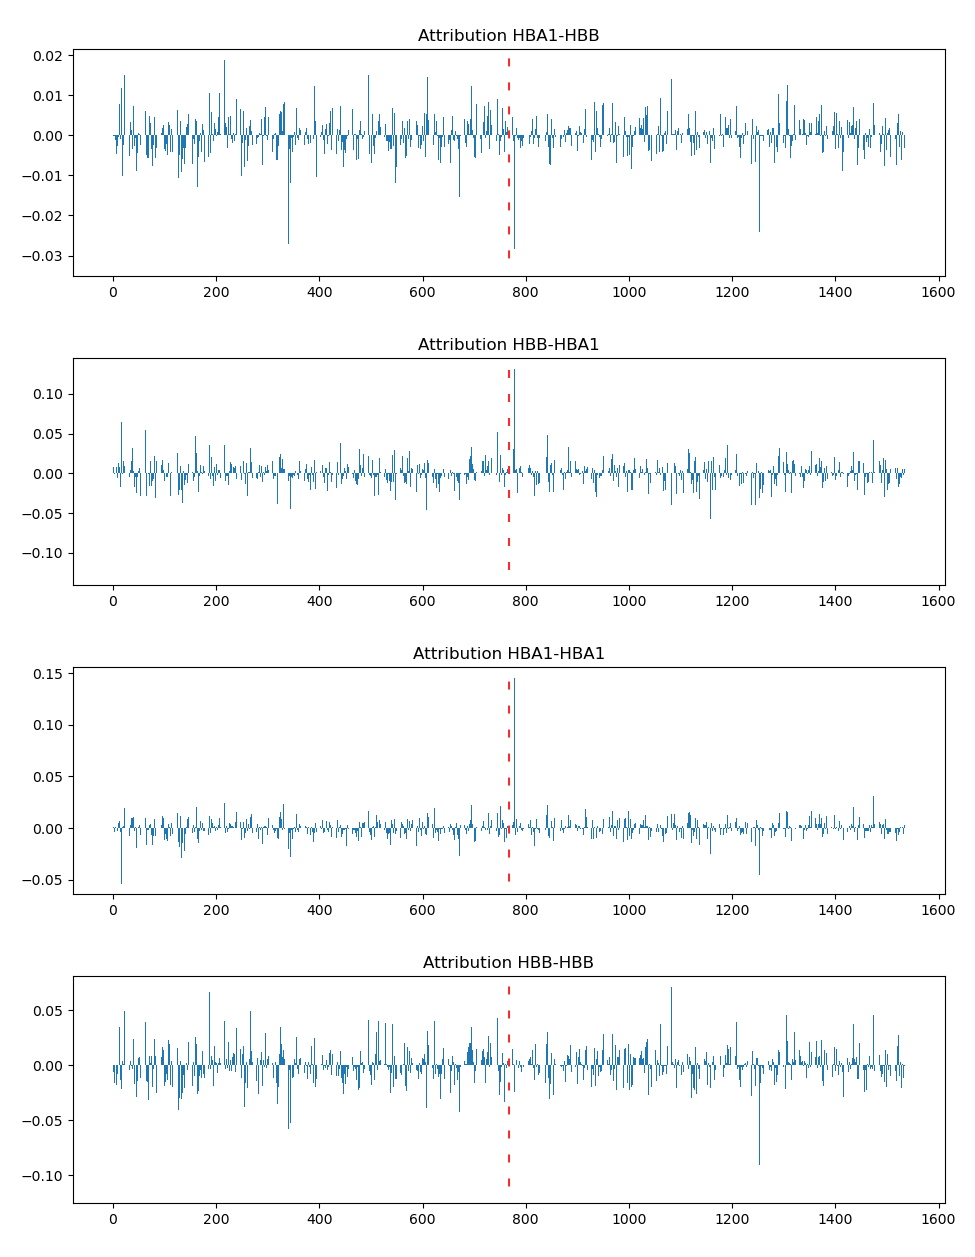
\includegraphics[width=\textwidth]{images/attribution_profil_annotated.png}
\caption{The attribution is given by the Integrated Gradient method for four inputs to the baseline MLP. The x-axis is the dimension and the y-axis is the attribution given to this dimension in the final decision of the model. The red dotted line is the delimitation between the embedding of the first and the second sequence. Even if there is a single physical HBA1-HBB interaction, the HBA1-HBB, and HBB-HBA1 inputs are distinct for the MLP, both are depicted in the figure.}
\label{attribution_profils}
\end{figure*}


The visualization of the "important" amino acid in the 3D structure of the complex is given in figure \ref{3D_HBB_HBA1_complex}. Despite the fact that the 3D shape is not easily understandable, we can find interesting structures that are at the surface of contact in the 3D space and contain important amino acids, like the ones highlighted by the blue circles. Nonetheless, further work on several examples, incorporating knowledge from biochemistry, is needed to evaluate the pertinence of this analysis. 

For now, we conclude that there seems to be no straightforward correlation between the "important" amino acids given by the analysis of the MLP and their position in the 3D space.

\begin{figure*}[ht]
\centering
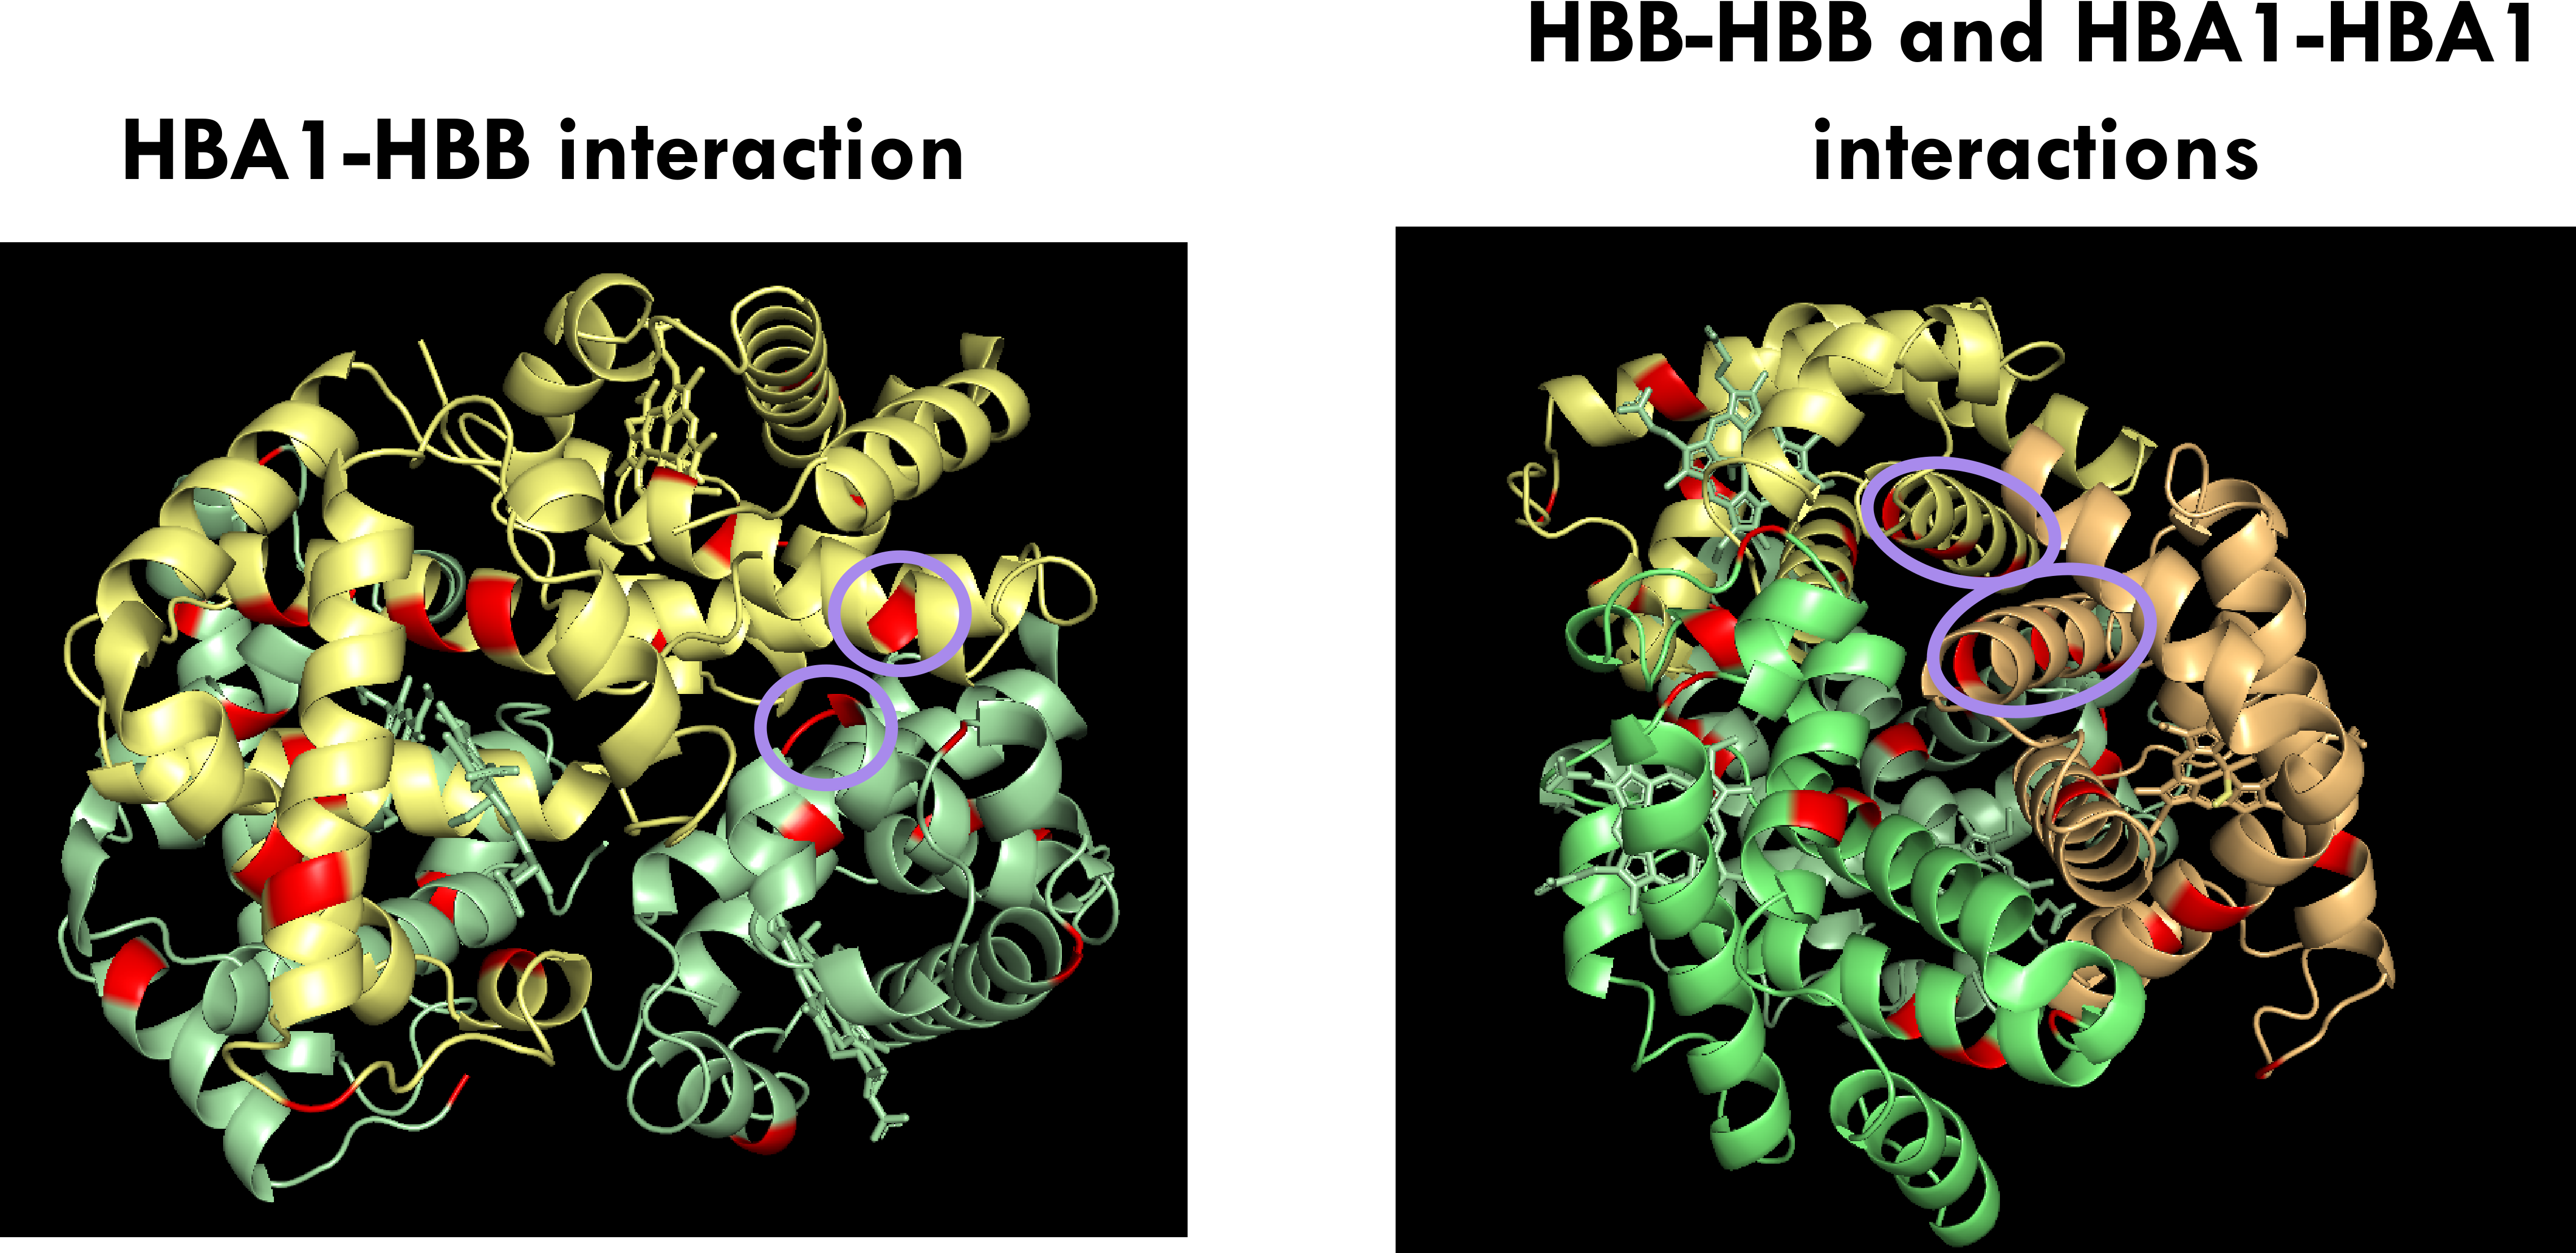
\includegraphics[width=0.8\textwidth]{images/struct_HBB_HBA1.png}
\caption{3D structure of the human hemoglobin, a complex of four proteins formed by two hemoglobin subunits alpha (HBA1, yellow) and two hemoglobin subunits beta (HBB, green). In red are the amino acids important for the classification by the MLP baseline model for different types of prediction. Highlighted in blue are "important" amino acids at the surface of contact for the relevant interaction.}
\label{3D_HBB_HBA1_complex}
\end{figure*}



\pagebreak
\FloatBarrier
\bibliographystyle{acl_natbib}
\bibliography{references}



\end{document}